\documentclass[12pt]{article}
\usepackage{amsmath,amssymb}
\usepackage{graphicx}
\usepackage{multirow}
\usepackage[usenames,dvipsnames]{xcolor}
\usepackage[utf8]{inputenc}
\usepackage[spanish,es-tabla]{babel}



\begin{document}

\title{TALLER 1}
\author{Miguel Angel Castillo Espitia}
\date{Febrero, 2019}
\maketitle

Puede escribir aquí. Las secciones del documento se pueden declarar como sigue:

\section{Teoría}
.\\
Cuando un cuerpo se desplaza cerca de la superficie de la tierra, experimenta el campo gravitacional de esta como una fuerza constante. Dado que no se le ejercen más fuerzas a su trayectoria, podemos definir su trayectoria en un marco de coordenadas que llamaremos (x,y). Las ecuaciones de movimiento en este marco de coordenadas son las siguientes:\



\begin{equation}
  \begin{aligned}
	  {x(t)}={x}_{0}+{v}_{x0}{t}
	  \label{eq1}
  \end{aligned}
\end{equation}

\begin{equation}
  \begin{gathered}
	  {y(t)}={y}_{0}+{v}_{y0}{t}-\frac{g}{2}{t^{2}}
	  \label{eq2}
  \end{gathered}
\end{equation}


  
\section{Experimento}

El experimento se basa en capturar un video en donde se muestre la caída de un objeto de color sólido. Cuando la cámara esté centrada en el trasfondo, procedemos a colocar dos marcas de color sólido separadas por un metro, esto con el fin de hallar un factor de conversión de las unidades de distancia de la imágen(pixeles) a metros.

\ref{graph1}:
\begin{figure}[h]
	\centering
	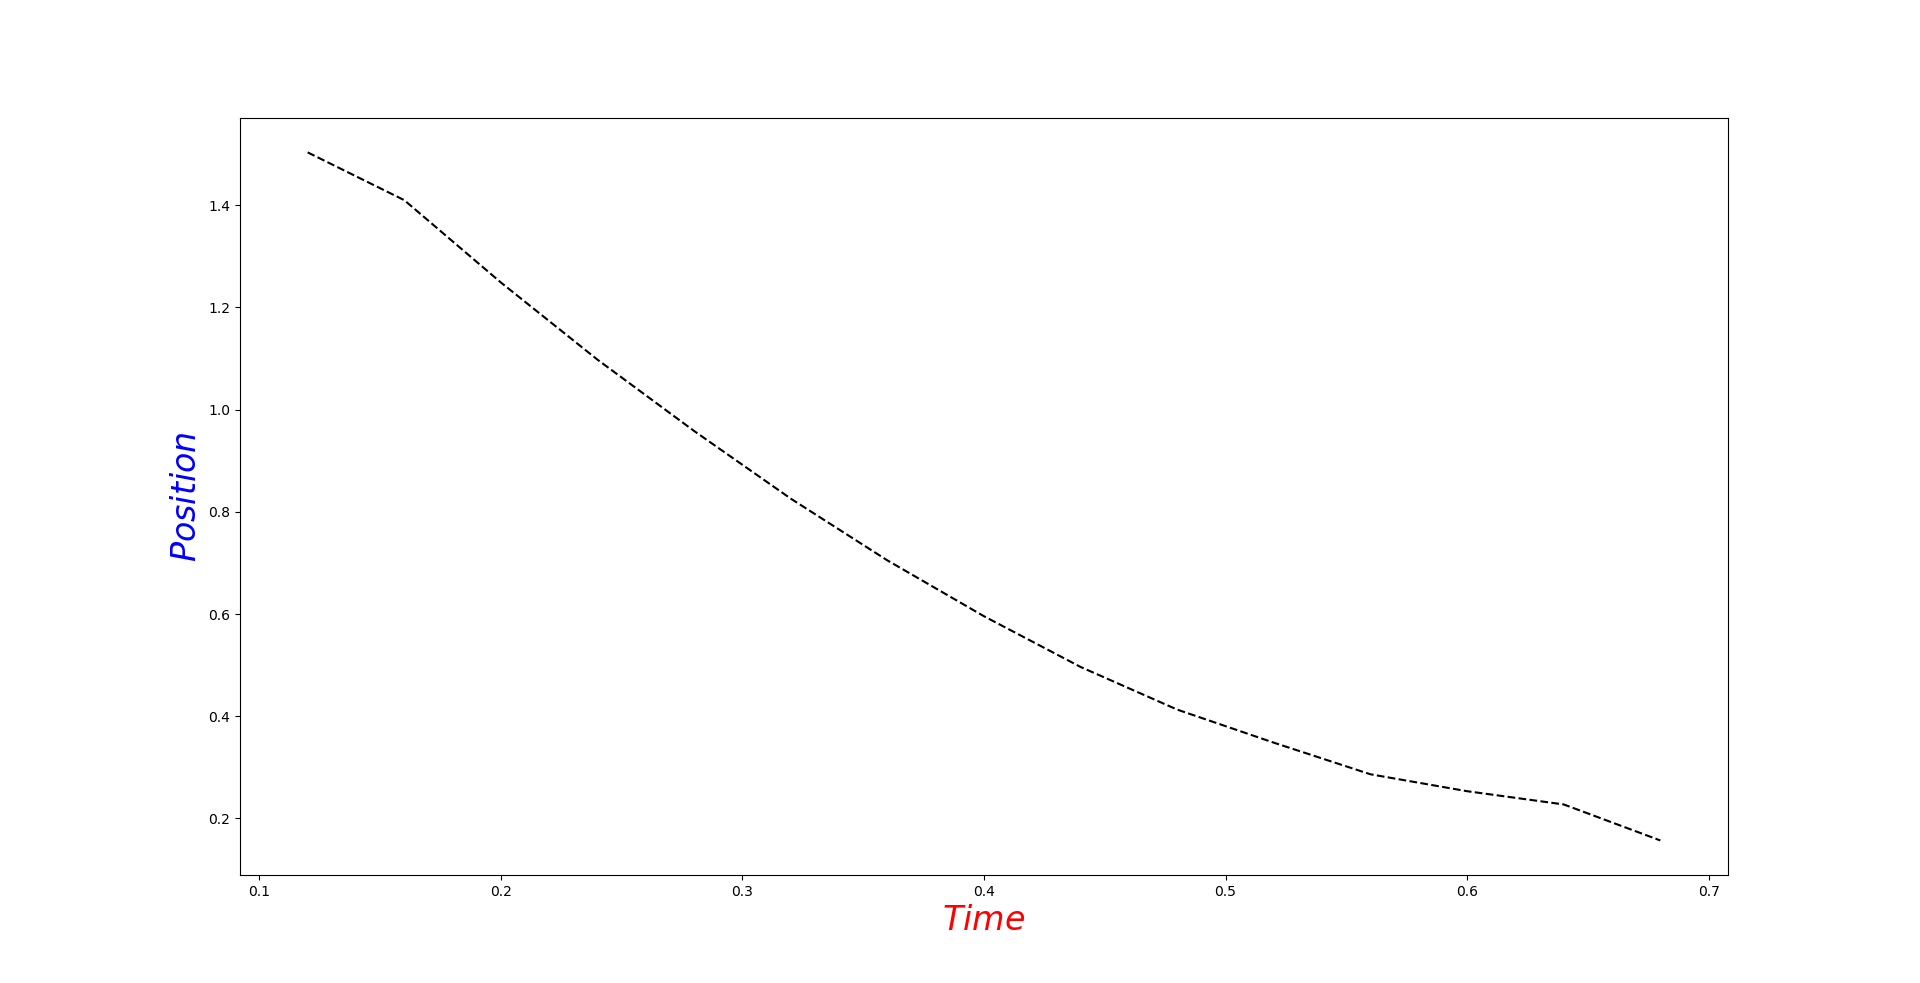
\includegraphics[scale=0.1]{Grafica.png}
	\caption{Esta es una figura.}
	\label{graph1}
\end{figure}
Describa el experimento. Enuncie los resultados del mismo, con tablas y figuras en lo posible.
Así se define una tabla, como Tabla \ref{table1}:
\begin{table}[h]
	\centering
	\begin{tabular}{|c|c|c|}
		\hline
		dato & dato & dato \\
		\hline
		dato & dato & dato \\
		\hline
		dato & dato & dato \\
		\hline
	\end{tabular}
	\caption{Esta es una tabla.}
	\label{table1}
\end{table}
\section{Análisis}
Discuta las observaciones que se hicieron y las comparaciones entre teoría, simulación y experimento. Un párrafo por cada observación.

\begin{thebibliography}{}

\bibitem{milibro}
  S. Carnot, {\it Reflexions sur la puissance motrice du feu et sur les machines proper \`a d\'eveloper cette uissance}, Bachelier, Paris (1824)

\bibitem{Proesmans}
  K. Proesmans, C. Driesen, B. Cleuren and C. Van der Broeck, Phys. Rev. E {\bf 92}, 032105 (2015)
    
\end{thebibliography}

\end{document}
